\section{Modularity through Clients and Services, RPC}

\paragraph{Layers and Modules}
\begin{itemize}
\item Interpreters often organized in layers
\item Modules
  \begin{itemize}
  \item Components that can be separately designed / implemented
    / managed / replaced (\textit{Saltzer \& Kaashoek glossary})
  \item ``Instructions'' of higher-level interpreters
  \item Recursive: can be whole interpreters themselves!
  \end{itemize}
\end{itemize}


\paragraph{Isolating Errors: Enforced Modularity}
\textbf{Problem: What happens when modules fail
  with (unintended) errors?}

$\rightarrow$ only that particular module should fail rest of system
should still work (for this need enforced modularity)

\textbf{Example: Clients \& Services}
\begin{itemize}
\item Restrict communication to \textit{message only}
\item Client request / Service response (or reply)
\item Conceptually client and service in different computers
\end{itemize}

\textbf{Example: OS Virtualization}
\begin{itemize}
\item Create virtualized version of fundamental abstraction
\item Client and services remain isolated even on same computer
\item VMs: virtualize the virtualizer
\end{itemize}

\paragraph{RPC: Remote Procedure Call}
\begin{itemize}
\item Client-service request / response interactions
\item Automate marshalling and communication
\end{itemize}

\begin{figure}[h]
\begin{minipage}{1.0\linewidth}
  \begin{center}
    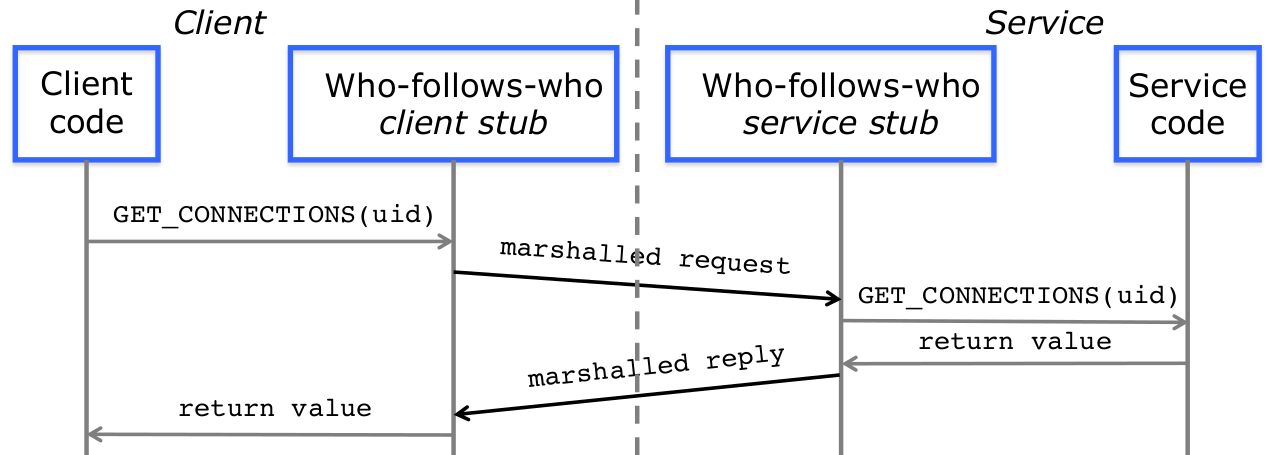
\includegraphics[scale=0.8]{graphics/rpc}
  \end{center}
  \end{minipage}
\end{figure}

\paragraph{RPC Semantics}
\begin{itemize}
\item \textbf{At-least-once}
  \begin{itemize}
  \item Operation is \textit{idempotent}
    (naturally occurs if side-effect free)
  \item Stub just retries operation $\rightarrow$ failures
    can still occur!
  \item Example: calculate SQRT
  \end{itemize}

\item \textbf{At-most-once}
  \begin{itemize}
  \item Operation does have side-effects
  \item Stub must ensure duplicate-free transmission
  \item Example: transfer \$100 from my account to yours
  \end{itemize}

\item \textbf{Exactly-once}
  \begin{itemize}
  \item possible for certain classes of failures
  \item Stub \& service keep track (\textit{durably}) of requests and
    responses
  \item Example: bank cannot develop amnesia!
  \end{itemize}
\end{itemize}

\paragraph{How to achieve RPCs?}
\begin{itemize}
\item Special-purpose \textbf{request-reply protocol} e.g. DNS
  \begin{itemize}
  \item Developer must design protocol and marshalling scheme
  \end{itemize}

\item \textbf{Classic RPC} protocols, DCE, Sun RPC
  \begin{itemize}
  \item Special APIs and schemes for marshalling
  \end{itemize}

\item \textbf{RMI: Remote Method Invocation}
  \begin{itemize}
  \item RPCs for methods in OO languages
  \item Compiler-generated proxies
  \end{itemize}

\item \textbf{Web Services}
  \begin{itemize}
  \item many modes of communication possible, including RPC-style
    communication
  \item Tools available to compile proxies, e.g., JAX-WS
  \item Generic marshalling (e.g., XML, JSON, Protocol Buffers)
    over HTTP transport \\
    $\rightarrow$ \textbf{programming-language Independence}
  \end{itemize}
\end{itemize}

\paragraph{RPC and Naming}
\begin{itemize}
\item Most basic extension to the synchronous interaction pattern
  \begin{itemize}
  \item Avoid having to name the destination
  \item Ask where destination is
  \item then bind to destination
  \end{itemize}

\item Advantages:
  \begin{itemize}
  \item Development is independent of deployment properties \\
    (e.g. network address)
  \item more flexibility
    \begin{itemize}
    \item change of address
    \end{itemize}
  \item Can be combined with
    \begin{itemize}
    \item Load balancing
    \item Monitoring
    \item Routing
    \item Advanced service search
    \end{itemize}
  \end{itemize}
\end{itemize}

\begin{figure}[h]
  \begin{minipage}{1.0\linewidth}
    \begin{center}
      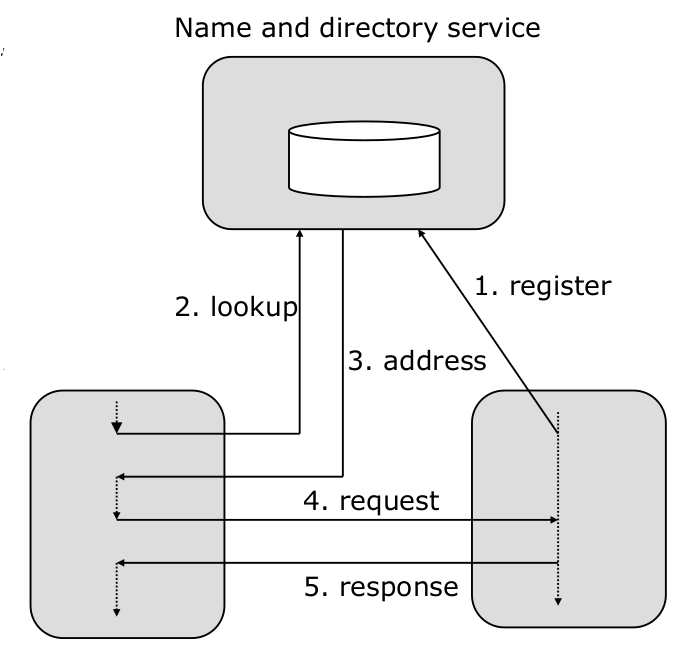
\includegraphics[scale=0.15]{graphics/naming}
    \end{center}
  \end{minipage}
\end{figure}

\paragraph{Common Issues in Designing Services}
\begin{itemize}
\item Consistency
  \begin{itemize}
  \item How to deal with \textit{updates} from multiple clients?
  \end{itemize}
\item Coherence
  \begin{itemize}
  \item How to refresh caches while respecting consistency?
  \end{itemize}
\item Scalability
  \begin{itemize}
  \item What happens to resource usage if we increase the
    \#clients or the \#operations?
  \end{itemize}
\item Fault Tolerance
  \begin{itemize}
  \item Under what cirumstances will the service be unavailable?
  \end{itemize}
\end{itemize}

\paragraph{Other Examples of Services}
\begin{itemize}
\item File systems: NFS, GFS
\item Object stores: Dynamo, PNUTS
\item Database: relational DB
\item Configuration: Zookeeper
\item Even whole computing clouds!
  \begin{itemize}
  \item Infrastructure-as-a-service (IaaS): e.g. Amazon EC2
  \item Platform-as-a-service (PaaS): e.g. Windows Azure
  \item Software-as-a-service (SaaS): e.g. Salesforce, Gmail
  \end{itemize}
\end{itemize}

\section{Techniques for Performance}

\paragraph{Motivation: Abstractions, Implementation and Performance}
Let $I_1$ and $I_2$ be two implementations of an abstraction

\begin{itemize}
\item Examples
  \begin{itemize}
  \item Web service with or without HTTP proxies
  \item Virtual memory with or without paging
  \item Transactions via concurrency or serialization
  \end{itemize}
\end{itemize}

$\Rightarrow$ \textbf{How can we choose between $I_1$ and $I_2$?}

\paragraph{Performance Metrics}
\begin{itemize}
\item \textbf{latency:} The delay between a change at the input to a
  system and the corresponding change at its output. From
  the client/service perspective, the latency of a request is the
  time from issuing the request until the time the response
  is received from the service.

\item \textbf{throughput:} Is a measure of the rate of useful work
  done by a service for some given workload of requests.
  If processing is serial, then throughput is inversely
  proportional to the average time to process a single request

  $$ throughput = \frac{1}{latency} $$

  If processing is concurrent, then no direct relationship between
  latency and throughput.

\item \textbf{scalability:} Scalability is the property of a system to handle a growing amount of work by adding resources to the system

\item \textbf{overhead:} In a layered system, each layer may have
  a different view of the capacity and utilization of the underlying
  resources. Each layer considers what the layer below it do to
  be \textit{overhead} in time and space, what the
  layers above it do to be \textit{useful work}.

\item \textbf{utilization:} The percentage of capacity used
  for a given workload

\item \textbf{capacity:} Any consistent measure of the size or amount
  of a resource.
\end{itemize}

\paragraph{How can we improve performance?}
\begin{itemize}
\item \textbf{Fast-path coding}
  \begin{itemize}
  \item Split processing into two code paths
  \item One optimized for common requests $\rightarrow$ fast path
  \item One slow but comprehensive path for all other
    requests $\rightarrow$ slow path
  \item Example: Caching
  \end{itemize}
\end{itemize}

\begin{figure}[h]
  \begin{minipage}{1.0\linewidth}
    \begin{center}
      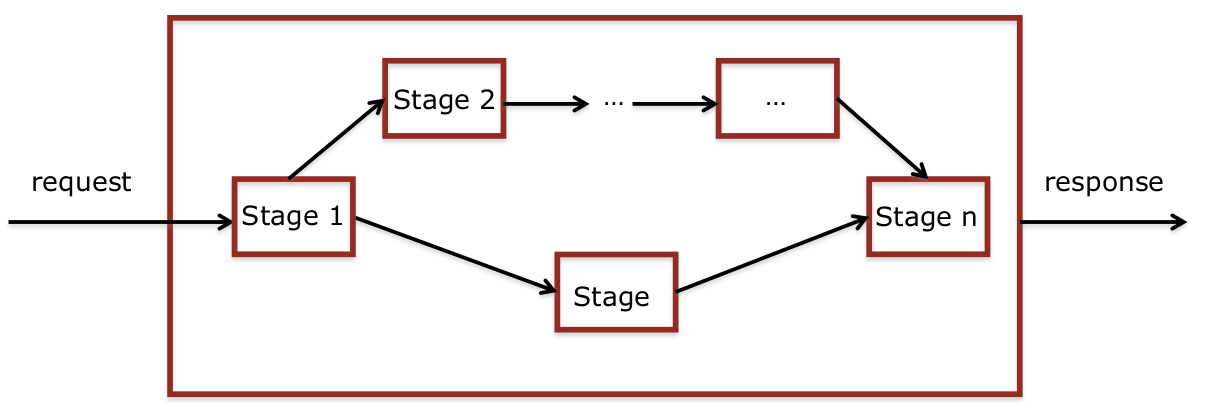
\includegraphics[scale=0.2]{graphics/fast_path.png}
    \end{center}
  \end{minipage}
\end{figure}

\begin{itemize}
\item \textbf{Batching}
  \begin{itemize}
  \item Run multiple requests at once
  \item Example: batch I/Os and use elevator algorithm
  \item May improve latency and throughput
  \end{itemize}
\end{itemize}

\begin{itemize}
\item \textbf{Dallying}
  \begin{itemize}
  \item Wait until you accumulate some requests and then run them
  \item Example: group commit
  \end{itemize}
\end{itemize}

\begin{itemize}
\item \textbf{Concurrency}
  \begin{itemize}
  \item Run multiple requests in different threads
  \item May improve both throughput and latency, but must
    be careful with locking (overhead), correctness
  \item Can be hidden under abstractions
    (e.g. MapReduce, transactions)
  \item Example: different web requests run in different threads
    or even servers
  \end{itemize}
\end{itemize}

\begin{itemize}
\item \textbf{Speculation}
  \begin{itemize}
  \item Guess the next requests and run them in advance
  \item May overlap expensive operations, instead of
    waiting for their completion
  \item Example: prefetching
  \end{itemize}
\end{itemize}

% LocalWords:  Modularity RPC Saltzer Kaashoek modularity virtualized
% LocalWords:  VMs virtualize virtualizer marshalling SQRT RPCs DNS
% LocalWords:  DCE APIs RMI OO JAX WS JSON Scalability cirumstances
% LocalWords:  NFS GFS PNUTS IaaS PaaS SaaS Gmail scalability
% LocalWords:  MapReduce prefetching
